% !TeX spellcheck = en_GB
% %%% ***************** CHAPTER INTRODUCTION ***************** %%%
\chapter{Introduction}
\label{ch:intro}
%%%%%%%%% INTRODUCTION %%%%%%%%%%%%%%
Global warming is predicted to cause an increased frequency of extreme weather events and heat waves, droughts, heavy rains or extremely high winds \citep{hansen_warmer_2014}. Weather and climate extremes can have serious effects on human society and infrastructure, as well as on ecosystems and wildlife.
Precipitation observations are important for hydrological, climate and weather research, as more than one-sixth of the world's population receives water from glaciers and seasonal snow packs \citep{barnett_potential_2005}. Severe weather events are mostly in the focus of media reports with respect to global warming \citep{meehl_introduction_2000}. Understanding and predicting the impact of extreme weather events is one of the grand challenges of current climate research \citep{stocker_working_2013,field_summary_2014}.
\par\medskip
\noindent
This work focuses on the extreme weather event during Christmas 2016, and the snow measurements and ensemble model forecasts taken at the measurement site Haukeliseter (\SI{991}{\metre} above sea level) in Southern Norway. The Christmas storm 2016, named 'Urd' by the Norwegian Meteorological Institute (Met-Norway), and had a large impact on Eastern, Southern, and Western Norway.  %\citep{olsen_ekstremvaerrapport._2017}. 
%Storms with high wind speed and precipitation amount are expected to occur approximately every five years. 
The financial costs associated with the Christmas storm 2016 are estimated to about 180 million Norwegian kroner. 'Urd' led to major traffic problems for cars, trains, ferries and air planes. Most mountain crossings were kept closed during Christmas 2016 \citep{olsen_ekstremvaerrapport._2017}. An increase in temperature and therefore a change of frozen to liquid precipitation followed an increase in avalanche danger. In addition, 40 emergency power stations failed during the extreme event affecting around 70.000 households (\Cref{fig:news}).
%a power blackout of around 70.000 households where 40 emergency power stations failed during the extreme weather (\Cref{fig:news}). 
Since people are affected by extreme weather it is important to accurately measure and forecast severe storms. The use of accurate observations will lead to better performing weather forecast models, which rely heavily on observations \citep{joos_influence_2012}. 
%%% images from Twitter and news %%%%%%%%%%%%%%%%%%%%%%%%%%%%%%%%%%%%%
% !TeX spellcheck = en_GB
\begin{figure}[t!]
	\centering
	\begin{subfigure}[b]{0.49\textwidth}
		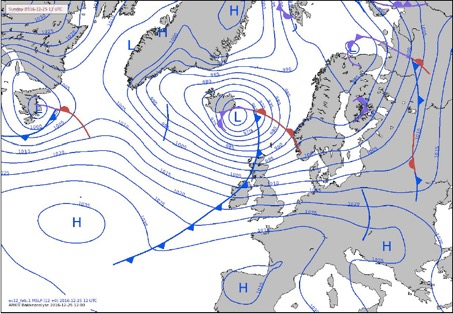
\includegraphics[width=\textwidth]{./fig_introduction/Ana_2512_12UTC.jpg}
		\caption{}\label{fig:ana_YR}
	\end{subfigure}
\hfill
	\begin{subfigure}[b]{0.49\textwidth}
		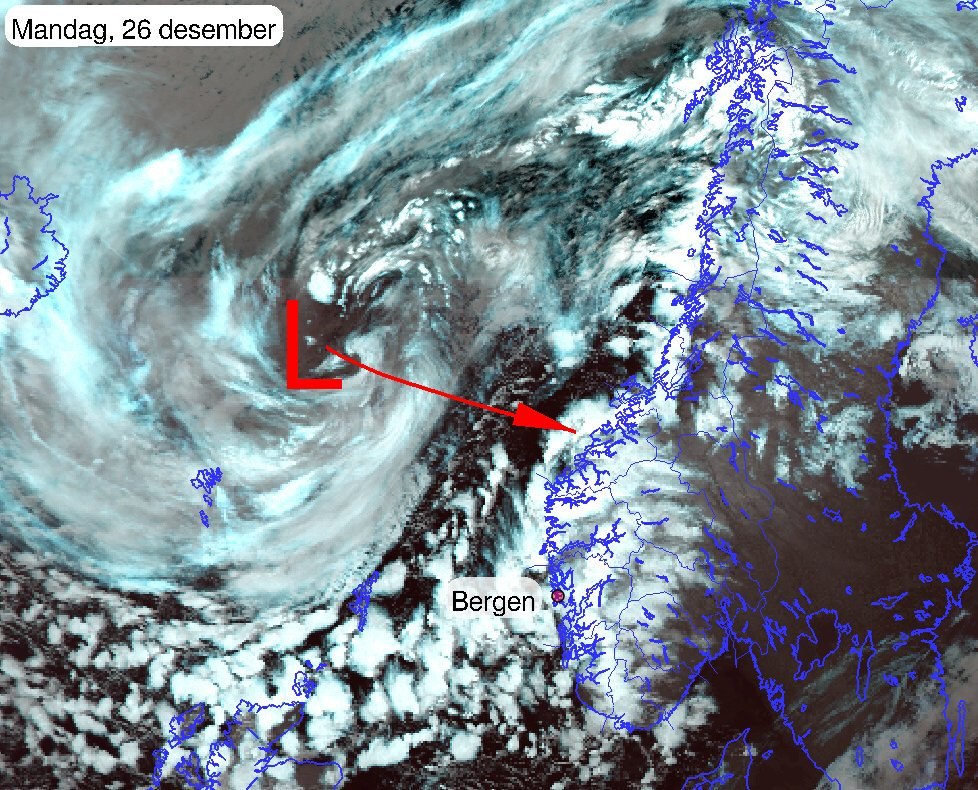
\includegraphics[trim={0cm 3.8cm 0cm 0cm},clip, width=\textwidth]{./fig_introduction/Twitter_26122016_0934AM.jpeg}
		\caption{}\label{fig:meteorologene_2612}	
	\end{subfigure}
	\begin{subfigure}[b]{0.49\textwidth}
		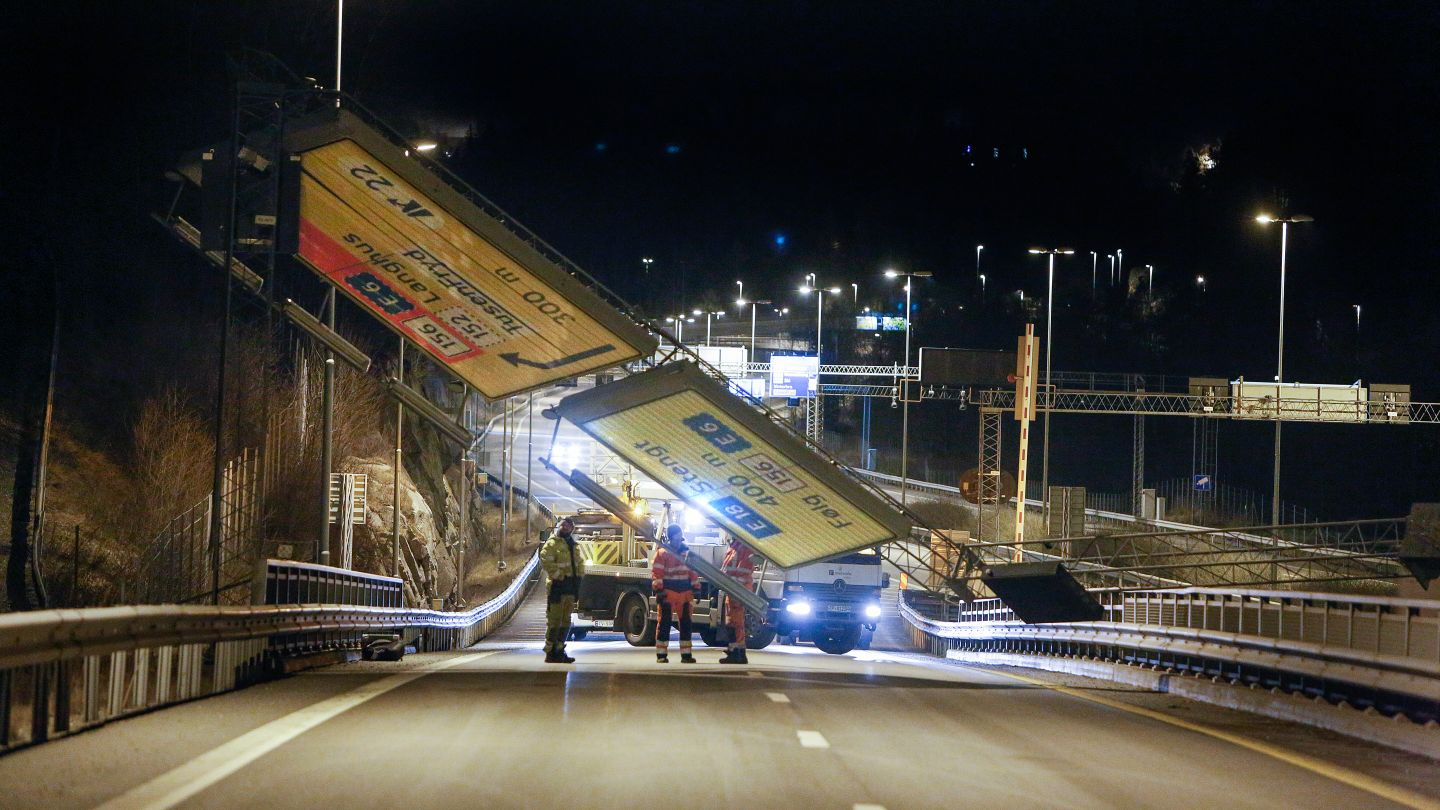
\includegraphics[width=\textwidth]{./fig_introduction/street_sign_2512.jpg}
		\caption{}\label{fig:street_sign}
	\end{subfigure}
\hfill
	\begin{subfigure}[b]{0.49\textwidth}
		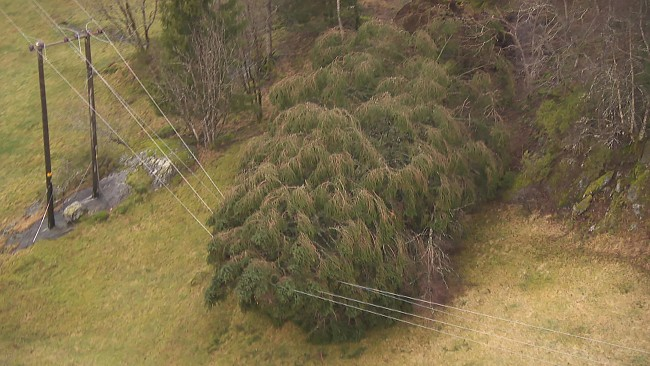
\includegraphics[width=\textwidth]{./fig_introduction/tree_nrk_2812.jpg}
		\caption{}\label{fig:tree_elec}
	\end{subfigure}
\caption{Weather situation during the extreme Christmas storm and impact on the infrastructure. In \protect\subref{fig:ana_YR}: Weather situation Sunday \SI{25}{\dec} at \SI{12}{\UTC} from the extreme weather report on Urd \citep{olsen_ekstremvaerrapport._2017}.
	\protect\subref{fig:meteorologene_2612}: Tweet from \cite{meteorologene_her_2016} on \SI{26}{\dec} at 9:34 am: Here comes \#Urd! The low pressure centre will hit M{\o}re og Romsdal, but the strongest wind comes south of Stad. \#S{\o}rNorge.
    \protect\subref{fig:street_sign} and \protect\subref{fig:tree_elec} show the consequences related to the high wind speeds during Christmas 2016.
	\protect\subref{fig:street_sign}: This traffic sign, ten meter long and four meter high was blown down during the storm, \citep{ruud_tonn_2016}.
	\protect\subref{fig:tree_elec}: Trouble maker: The extreme weather during Christmas created problems for the local infrastructure. \num{80.000} households were without electricity during the storm, \citep{farestveit_80.000_2016}.} \label{fig:news}
\end{figure}
%%%%%%%%%%%%%%%%%%%%%%%%%%%%%%%%%%%%%%%%%%%%%%%%%%%%%%%%%%%%%%%%%%%%%%%%%%
% previous background
\par\medskip
\noindent
It has long been known that measuring precipitation, especially in the form of snow, is difficult. Winter precipitation measurement shows biases of more than \SI{100}{\percent} between different gauge observation networks and different regions leading to different habit and size of frozen aggregates \citep{kochendorfer_analysis_2017}. An adjustment transfer function for single fence gauges represents a capture efficiency as a function of air temperature and wind speed to delimit the error of measured snowfall.
% The local climate changes from station to station lead to different habit and size of frozen aggregates \citep{kochendorfer_analysis_2017,wolff_derivation_2015}. %Measurement uncertainties can be caused by the instrument itself, which varies with wind speed, gauge wind shielding, shape, size, phase, and fall velocity of hydrometeors \citep{kochendorfer_analysis_2017,wolff_derivation_2015}. 
%Additionally, u
Uncertainties in precipitation measurements under windy conditions can affect water balance calculation and the calibration of remote sensing algorithms \citep{wolff_derivation_2015}. 
% \\
%Since wind has an influence on frozen precipitation, a WMO (World Meteorological Organization) precipitation analysis between 1987 and 1993 recommended that the double-fence inter-comparison reference should be used as a reference for snow measurements \citep{goodison_wmo_1998}. An adjustment for unshielded and single-shielded precipitation gauges followed in 2010. The 
%%%%%%%%%%%%%%%%%%%%%%%%%%%%%%%%%%%%%%%%%%%%%%%%%%%%%%%%%%%%%%%%%%%%%%%%%%%%%%%%%%%%%%%%%%%%
\par\medskip
\noindent
Estimates of snowfall from radar reflectivities are non-unique.  This means that a given reflectivity can yield very different estimates of snowfall depending upon the precise microphysical assumptions used in the retrieval scheme. \citet{kulie_utilizing_2009}, for example, used the CloudSat Cloud Profiling Radar (CPR) to estimate global snowfall from a year of reflectivity data. They found that snowfall estimates critically depend on assumed snowfall particle size distribution, shape and fall speed.  They concluded that the use of traditional Z-S relationships in which snow (S) is derived only from knowledge of radar reflectivity (Z) can lead to large retrieval uncertainties for a given snowstorm.  Subsequent studies have tried to incorporate scene dependent microphysical information into the retrieval scheme. \citet{wood_estimation_2011} incorporated a particle size distribution-temperature relationship information into the CloudSat operational snowfall retrieval scheme to help reduce retrieval non-uniqueness.  In turn, \citet{cooper_variational_2017} used in-situ estimates of snowflake PSD and habit from ground-based instrumentation to explore surface snowfall retrieval performance at Barrow, Alaska. They found reasonable agreement within \SI{20}{\percent} of nearby snow gauge measurements. Given limited snowfall observed at Barrow, Alaska, it was difficult to come to any definitive conclusions about retrieval performance.
%%%%%%%%%%%%%%%%%%%%%%%%%%%%%%%%%%%%%%%%%%%%%%%%%%%%%%%%%%%%%%%%%%%%%%%%%%%%%%%%%%%%%%%%%%%%
\par\medskip
\noindent
With the increasing expansion of computational power, developments of high-resolution numerical weather forecasting models with $\le$\SI{4}{\km} scales can be able to represent small-scale phenomena, such as convective dynamics \citep{gowan_validation_2018}. 
Information on magnitudes and location of maximum precipitation amount and wind speed is of significant importance when warnings are published by meteorological services for severe weather events and for further use, e.g. the Norwegian Water Resources and Energy Directorate's hydrological model for flooding and avalanche risk.
The ability to use high-resolution models is also followed by various challenges, such as physical parametrisation schemes, accurate representation of topography such as in Norway, and data assimilation of high-resolution data \citep{sun_convective-scale_2005}. 
% \\
%The weather forecast in Scandinavia includes continental, maritime and polar conditions. Norway has complex topography, gradients in mountain terrain, as well as highly resolved coastline, which can complicate local weather forecasting of precipitation, wind, and temperature \citep{muller_arome-metcoop:_2017}. %\citet{colle_1314_2005,garvert_1314_2005,schwartz_reproducing_2014}, for example, have shown, that simulations of orographic precipitation can be improved in mountainous terrain for horizontal grid spacing below \SI{4}{\km}. 
Uncertainties on a convective scale can lead to a rapid error growth \citep{lorenz_atmospheric_1969}, hence high-resolution ensemble prediction makes it possible to estimate the forecast uncertainty by performing several model runs, each with different initial conditions. %\citep{gowan_validation_2018}
\\
The Meteorological Cooperation on Operational Numerical Weather Prediction (MetCoOp) Ensemble Prediction forecast (MEPS) has been operational at Met-Norway since November 2016. The ensemble prediction system uses the previous deterministic AROME-MetCoOp, a version of the Mèteo-France Applications of Research to Operations at MEsoscale (AROME). In addition to the deterministic forecast, nine perturbed ensemble members are initialised in MEPS. 
%The newly developed ensemble prediction systems from Met-Norway is used to analyse the extreme winter storm during Christmas 2016.
\par\medskip
\noindent
The Christmas storm in 2016 is an excellent test case for analysing unique available precipitation observations at Haukeliseter, Norway, together with the newly available ensemble system, MEPS.
% \\
% Steve re-wrote
Haukeliseter has been a World Meteorological Organization (WMO) measuring station with single and double fence precipitation instruments since 2010. During winter 2016/17, the Haukeliseter site also housed a Micro Rain Radar (MRR), Multi-Angle Snow Camera \citep[MASC;][]{garrett_fall_2012}, and Precipitation Imaging Package (PIP) as part of US National Science Foundation (NSF) funded field campaign. Such a combination of radar and in-situ microphysical observations provided an ideal mean to estimate vertical precipitation profiles of snowfall rate and snow water content as in \citet{cooper_variational_2017}. Such profiles, in turn, could be used to evaluate the representation of snow water in the weather prediction forecasts for storms such as Urd. \citet{joos_influence_2012} stressed the need for improved observational constraints of the vertical profile of precipitation for forecast models. They showed that storm development in a regional forecast model depends upon whether or not the location of the precipitation is correctly simulated.  The precise profile of precipitation determines the latent heating profile, which can lead to either potential vorticity generation or destruction. 
\\
This thesis is investigating if the ensemble prediction system is able to forecast the variation of an extreme winter event such as 'Urd' and if the forecast model is able to predict large scale weather systems %phenomena 
as well as frozen precipitation. Furthermore, the use of an ensemble prediction system will give the possibility to compare the variation of snowfall precipitation at the surface and in the vertical at Haukeliseter. Observations will help to compare MEPS model forecast to examine the following research questions: 
Does the regional model cover local affects associated with the topography surrounding the measurement site? How well does the model predict the surface snowfall at the Haukeliseter measurement site during the Christmas storm 2016? 
Are large scale synoptic weather systems resolved by MEPS?
Is there a difference between estimated surface accumulation for different optimal estimation assumptions and locations? 
\\
\\
The thesis is structured as following: %The next section provides the background for the motivation of this thesis.
\Cref{ch:Methods} gives an overview of the measurement site Haukeliseter and its instrumentation, followed by the theory and methodology on the optimal estimation retrieval as well as a description of the regional model MEPS. The data calculation for MEPS and the statistical analysis is presented in \Cref{sec:data_proc}.
Afterwards, the evolution of the 2016 extreme Christmas storm is investigated, using European Centre for Medium-Range Weather Forecasts (ECMWF) analysis maps.
%The 2016 extreme Christmas storm is analysed in \Cref{ch:weather_ana}. 
\Cref{ch:Res} analyse meteorological parameters at the surface to test if large scale weather systems were predicted at Haukeliseter.
Furthermore, %the section shows 
the comparison between the double fence gauge measurement and the retrieved snowfall amount at the surface is shown. Followed by an investigation about overestimation of surface precipitation amount by MEPS. Afterwards the retrieved snow water content is compared to MEPS simulations as well as the wind and snowfall related orographic influence is discussed.
%, analyse if large scale phenomena were predicted at Haukeliseter, and discuss overestimation of surface precipitation amount as well as the wind and snowfall related orographic influence.
The final chapter summarises the results and gives an outlook for research.
%%%%%%%%%%%%%%%%%%%%%%%%%%%%%%%%%%%%%%%%%%%%%%%%%%%%%%%%%%%%	
